%%
%% This is file `ubcsample.tex',
%% generated with the docstrip utility.
%
% The original source files were:
%
% ubcthesis.dtx  (with options: `ubcsampletex')
%% 
%% This file was generated from the ubcthesis package.
%% --------------------------------------------------------------
%% 
%% Copyright (C) 2001
%% Michael McNeil Forbes
%% mforbes@alum.mit.edu
%% 
%% This file may be distributed and/or modified under the
%% conditions of the LaTeX Project Public License, either version 1.2
%% of this license or (at your option) any later version.
%% The latest version of this license is in
%%    http://www.latex-project.org/lppl.txt
%% and version 1.2 or later is part of all distributions of LaTeX
%% version 1999/12/01 or later.
%% 
%% This program is distributed in the hope that it will be useful,
%% but WITHOUT ANY WARRANTY; without even the implied warranty of
%% MERCHANTABILITY or FITNESS FOR A PARTICULAR PURPOSE.  See the
%% LaTeX Project Public License for more details.
%% 
%% This program consists of the files ubcthesis.dtx, ubcthesis.ins, and
%% the sample figures fig.eps and fig.fig.
%% 
%% This file may be modified and used as a base for your thesis without
%% including the licence agreement as long as the content (i.e. textual
%% body) of the file is completely rewritten. You must, however, change
%% the name of the file.
%% 
%% This file may only be distributed together with a copy of this
%% program. You may, however, distribute this program without generated
%% files such as this one.
%% 


% This Sample thesis requires \LaTeX2e
\NeedsTeXFormat{LaTeX2e}[1995/12/01]
%\ProvidesFile{ubcsample.tex}[2015/05/31 v1.72 ^^J
% University of British Columbia Sample Thesis]
% This is the \documentclass[]{} command.  The manditory argument
% specifies the "flavour" of thesis (ubcthesis for UBC).  The
% optional arguments (in []) specify options that affect how the
% thesis is displayed.  Please see the ubcthesis documentation for
% details about the options.
%\documentclass[msc,oneside]{ubcthesis}
\documentclass[msc]{ubcthesis}
% this disables the cleardoublepage command
% this way, chapters can start on either the left or right page, not just the right page
\renewcommand{\cleardoublepage}{\clearpage}
%\usepackage[pass,paperwidth=8.5in,paperheight=11in]{geometry}
%\usepackage[
%        paperwidth=8.5in,
%        paperheight=11in,
%        % other options: a3paper, a5paper, etc
%        left=3.2cm,
%        right=2.5cm,
%        top=2.5cm,
%        bottom=2.5cm,
%        % use vmargin=2cm to make vertical margins equal to 2cm.
%        % us  hmargin=3cm to make horizontal margins equal to 3cm.
%        % use margin=3cm to make all margins  equal to 3cm.
%        ]
%{geometry}
\usepackage[
        paperwidth=8.5in,
        paperheight=11in,
        % other options: a3paper, a5paper, etc
        inner=3.2cm,
        outer=2.5cm,
        top=2.5cm,
        bottom=2.5cm,
        % use vmargin=2cm to make vertical margins equal to 2cm.
        % us  hmargin=3cm to make horizontal margins equal to 3cm.
        % use margin=3cm to make all margins  equal to 3cm.
        ]
{geometry}
%\pdfpageheight=11in
%\pdfpagewidth=8.5in
%
% To compile this sample thesis, issue the following commands:
% latex ubcsample
% bibtex ubcsample
% latex ubcsample
% latex ubcsample
% latex ubcsample
%
% To view use xdvi (on unix systems):
% xdvi ubcsample.dvi
%
% To make a postscript file, use dvips:
% dvips -o ubcsample.ps ubcsample.dvi
%
% To view the postscript file, use ghostview or gv (on unix systems):
% gv ubcsample.ps
%
%************************************************
% Optional packages.
%
% The use of these packages is optional, but they provide various
% tools for more flexible formating.  The sample thesis uses these,
% but if you remove the example code, you should be able to exclude
% these packages.  Only standard packages have been described here;
% they should be installed with any complete LaTeX instalation, but
% if not, you can find them at the Comprehensive TeX Archive Network
% (CTAN): http://www.ctan.org/
%

\usepackage{caption}
\usepackage{subcaption}

\usepackage{framed}

\usepackage{cancel}

% package for boxing multi-line equations
\usepackage{empheq}

%******** afterpage ***************************
% This package allows you to issue commands at the end of the current
% page.  A good use for this is to use the command
% \afterpage{\clearpage} right after a figure.  This will cause the
% figure to be inserted on the page following the current one (or on
% the current page if it will fit) but will not break the page in the
% middle.
\usepackage{afterpage}
\usepackage{xcolor}
%******** float *********************************
% This package allows you to customize the style of
% "floats"---floating objects such as figures and tables.  In
% addition, it allows you to define additional floating objects which
% may be included in a list similar to that produces by \listoftables
% and \listoffigures.  Common uses include introducing floats for
% programs and other code bits in Compute Science and Chemical Schema.
\usepackage{float}
\usepackage{amsmath,amssymb,bm}
%******** tocloft *******************************
% This package allows you to customize and define custom lists such
% as a list of programs or Chemical Scheme.  Note: if you use the
% subfigure package, you must specify that you do as an option here.
% The title option uses the default formatting.  We do not use this
% here as the default formatting is acceptable.  Use the float
% package instead unless you need the extra formatting control
% provided by tocloft.
%\usepackage[subfigure, titles]{tocloft}

%******** alltt *********************************
% The alltt package allows you to include files and have them
% formatted in a verbatim fashion.  This is useful for including
% source code from an additional file.
%\usepackage{alltt}

%******** listings ******************************
% The listings package may be used to include chunks of source code
% and has facilities for pretty-printing many languages.
%\usepackage{listings}

%******** longtable *****************************
% The longtable package allows you to define tables that span
% multiple pages.



\usepackage{longtable}

%******** graphics and graphicx *****************
% This allows you to include encapsulated postscript files.  If you
% don't have this, comment the \includegraphics{} line following the
% comment "%includegraphics" later in this file.
\usepackage{graphicx}

%******** subfigure *****************************
% The subfigure package allows you to include multiple figures and
% captions within a single figure environment.
%\usepackage{subfigure}

%******** here **********************************
% The here package gives you more control over the placement of
% figures and tables.  In particular, you can specify the placement
% "H" which means "Put the figure here" rather than [h] which means
% "I would suggest that you put the figure here if you think it looks
% good."
%\usepackage{here}

%******** pdflscape ********************************
% This allows you to include landscape layout pages by using the
% |landscape| environment.  The use of |pdflscape| is preferred over
% the standard |lscape| package because it automatically rotates the
% page in the pdf file for easier reading.  (Thanks to Joseph Shea
% for pointing this out.)
\usepackage{pdflscape}

%******** natbib ********************************
% This is a very nice package for bibliographies.  It includes options
% for sorting and compressing bibliographic entries.
\usepackage[numbers,sort&compress]{natbib}
%\usepackage{natbib}   % omit 'round' option if you prefer square brackets

%\usepackage{hyperref}
\usepackage[hidelinks]{hyperref}
%\usepackage[unicode=true,
%  colorlinks=true,
%  linktocpage,
%  linkbordercolor={0.5 0.5 1},
%  citebordercolor={0.5 1 0.5},
%  linkcolor=blue]{hyperref}


\usepackage[nameinlink]{cleveref}


% number figures globally instead of by chapter
\counterwithout{figure}{chapter}

% theorems
\usepackage{amsthm}
\theoremstyle{definition}
\newtheorem{definition}{Definition}
\newtheorem{theorem}[definition]{Theorem}

% for clever referencing, i.e. references equations as e.g.: eq. (1.1), particularly useful together with hyperref (which is automatically loaded by jcappub)

%******** psfrag ******************************
% This allows you to replace text in postscript pictures with formated
% latex text.  This allows you to use math in graph labels
% etc. Uncomment the psfrag lines following the "%psfrag" comment
% later in this file if you don't have this package.  The replacements
% will only be visible in the final postscript file: they will be
% listed in the .dvi file but not performed.
%\usepackage{psfrag}
%\usepackage[margin=0.5in]{geometry}
%******** hyperref *****************************
% Please read the manual:
% http://www.tug.org/applications/hyperref/manual.html
%
% This adds hyperlinks to your document: with the right viewers (later
% versions of xdvi, acrobat with pdftex, latex2html etc.) this will
% make your equation, figure, citation references etc. hyperlinks so
% that you can click on them.  Also, your table of contents will be
% able to take you to the appropriate sections.  In the viewers that
% support this, the links often appear with an underscore.  This
% underscore will not appear in printed versions.
%
% Note: if you do not use the hypertex option, then the dvips driver
% may be loaded by default.  This will cause the entries in the list
% of figures and list of tables to be on a single line because dvips
% does not deal with hyperlinks on broken lines properly.
%
% NOTE: HYPERREF is sensitive to the ORDER in which it is LOADED.
% For example, it must be loaded AFTER natbib but BEFORE newly
% defined float environments.  See the README file with the hyperref
% for some help with this.  If you have some very obscure errors, try
% first disabling hyperref.  If that fixes the problem, try various
% orderings.
%
% Note also that there is a bug with versions before 2003/11/30
% v6.74m that cause the float package to not function correctly.
% Please ensure you have a current version of this package.  A
% warning will be issued if you leave the date below but do not have
% a current version installed.
%
% Some notes on options: depending on how you build your files, you
% may need to choose the appropriate option (such as [pdftex]) for the
% backend driver (see the hyperref manual for a complete list).  Also,
% the default here is to make links from the page numbers in the table
% of contents and lists of figures etc.  There are other options:
% excluding the [linktocpage] option will make the entire text a
% hyperref, but for some backends will prevent the text from wrapping
% which can look terrible.  There is a [breaklinks=true] option that
% will be set if the backend supports (dvipdfm for example supports
% it but does not work with psfrag.)
%
% Finally, there are many options for choosing the colours of the
% links.  These will be included by default in future versions but
% you should probably consider changing some now for the electronic
% version of your thesis.
%\usepackage[unicode=true,
%  linktocpage,
%  linkbordercolor={0.5 0.5 1},
%  citebordercolor={0.5 1 0.5},
%  linkcolor=blue]{hyperref}

% If you would like to compile this sample thesis without the
% hyperref package, then you will need to comment out the previous
% \usepackage command and uncomment the following command which will
% put the URL's in a typewriter font but not link them.
%\newcommand\url[1]{\texttt{#1}}

%%%%%%%%%% CUSTOM COMMANDS


% order
\newcommand{\Od}[1]{\mathcal{O}{\left(#1\right)}}

% bras and kets
\newcommand{\bra}[1]{\left\langle#1\right|}
\newcommand{\ket}[1]{\left|#1\right\rangle}
\newcommand{\braket}[2]{\left\langle#1|#2\right\rangle}

% main basis used for bipartite system
\newcommand{\bket}[2]{\ket{#1\;#2}}
\newcommand{\bbra}[2]{\bra{#1\;#2}}

% the Hilbert space
\newcommand{\hilb}{\mathcal{H}}

% quantum operators
\newcommand{\op}[1]{\hat{#1}}

% imaginary and real parts
\renewcommand{\Im}{\operatorname{Im}}
\renewcommand{\Re}{\operatorname{Re}}

% trace
\newcommand{\Tr}[1]{\operatorname{Tr}\left(#1\right)}

% expectation value
\newcommand{\ex}{\mathbb{E}\,}

%******** setspace *******************************
% The setspace package allows you to manually set the spacing of the
% file.  UBC may require 1.5 spacing for microfilming of theses.  In
% this case you may obtain this by including this package and issuing
% one of the following commands:
%\usepackage{setspace}
%\singlespacing
%\onehalfspacing
%\doublespacing

% These commands are optional.  The defaults are shown.  You only
% need to include them if you need a different value
\institution{The University Of British Columbia}

% If you are at the Okanagan campus, then you should specify these
% instead.
%\faculty{The College of Graduate Studies}
%\institutionaddress{Okanagan}
\faculty{The Faculty of Science}
\institutionaddress{Vancouver}
\degreetitle{Bachelor of Science}

% You can issue as many of these as you have...
%\previousdegree{B.Sc., University of British Columbia, year}
%\previousdegree{M.Sc., The University of British Columbia, 2022}
%\previousdegree{Ph.D., Massachusetts Institute of Technology, 2005}

% You can override the option setting here.
% \degreetitle{Jack of All Trades}

% These commands are required.
\title{Entropy Growth in Quantum Mechanics}
%\subtitle{With a Subtitle}
\author{Duncan MacIntyre}
%\copyrightyear{2000}
\submitdate{\monthname\ \number\year} % The "\ " is required after
                                      % \monthname to prevent the
                                      % command from eating the space.
\program{Combined Honours in Physics and Mathematics}

% These commands are presently not required for UBC theses as the
% advisor's name and title are not presently required anywhere.
%\advisor{Ariel R.~Zhitnitsky}
%\advisortitle{Professor of Physics}

% One might want to override the format of the section and chapter
% numbers.  This shows you how to do it.  Note that the current
% format is acceptable for submission to the FoGS: If you wish to modify
% these, you should check with the FoGS explicity. prior to making
% the modifications.
\renewcommand\thepart         {\Roman{part}}
\renewcommand\thechapter      {\arabic{chapter}}
\renewcommand\thesection      {\thechapter.\arabic{section}}
\renewcommand\thesubsection   {\thesection.\arabic{subsection}}
\renewcommand\thesubsubsection{\thesubsection.\arabic{subsubsection}}
\renewcommand\theparagraph    {\thesubsubsection.\arabic{paragraph}}
\renewcommand\thesubparagraph {\theparagraph.\arabic{subparagraph}}

\setcounter{tocdepth}{2}
\setcounter{secnumdepth}{2}
%\newcommand{\arefe}[1]{{\textcolor{cyan}{#1}}}
% Here is an example of a "Program" environment defined with the
% "float" package.  The list of programs will be stored in the file
% ubcsample.lop and the numbering will start with the chapter
% number.  The style will be "ruled".
\floatstyle{ruled}
\newfloat{Program}{htbp}{lop}[chapter]

% Here is the start of the document.
\begin{document}

%% This starts numbering in Roman numerals as required for the thesis
%% style and is mandatory.
\frontmatter

%%% The order of the following components should be preserved.  The order
%%% listed here is the order currently required by FoGS:        \\
%%% Title (Mandatory)                                           \\
%%% Preface (Manditory if any collaborator contributions)       \\
%%% Abstract (Mandatory)                                        \\
%%% List of Contents, Tables, Figures, etc. (As appropriate)    \\
%%% Acknowledgements (Optional)                                 \\
%%% Dedication (Optional)                                       \\

\maketitle                      %% Mandatory

\clearpage

%%%THESIS APPROVAL PAGE - REQUIRED AS PART OF YOUR COMPLETED THESIS

%%%%%%% UBC FoGPS Requires the following statements at the beginning of the thesis. There is a (separate) thesis approval form that has to be signed and dated by the same individuals listed here as approving the thesis. You will have to get ensure that your department submits that approval form before you will be able to create an account and upload your thesis onto ciRCle. 
\noindent
The following individuals certify that they have read, and recommend to the Faculty of Science for acceptance, the thesis entitled:

\bigskip\noindent
\textbf{Entropy Growth in Quantum Mechanics}



\bigskip\noindent
submitted by 
\textbf{Duncan MacIntyre}
in partial fulfillment of the requirements for
the degree of 
\textbf{Bachelor of Science}
\bigskip\noindent
in the program	\textbf{Combined Honours in Physics and Mathematics}


\bigskip\noindent
%\textbf{[Include titles, departments, and universities, or titles and organizations. Remember to remove ALL material in square brackets [  ] before adding the page to your thesis.] Modify the examining committee to adapt to your case.}

\bigskip\noindent
\textbf{Examining Committee:}

\bigskip\noindent
Supervisor: Gordon Semenoff

%\bigskip\noindent
%Co-supervisor: \hrulefill

%\bigskip\noindent
%Supervisory Committee Member: \hrulefill

\bigskip\noindent
Additional Examiner: Panos Betzios

%\bigskip\noindent
%Additional Supervisory Committee Members: 

%\bigskip\noindent
%Supervisory Committee Member:\hrulefill



\clearpage
\newpage
\null
\newpage

\begin{abstract}                %% Mandatory -  maximum 350 words

When a small perturbation \(\lambda \op{V}\) is added to a Hamiltonian \(\op{H}_0\), the Von Neumann entropy of a subsystem may change as a result. I study this change in entropy. In particular, I derive a general expression for the change in entropy based on perturbative corrections to the eigenvalues of the reduced density operator. It shows that the entropy of a mixed state will never decrease provided (1) there exist component states with zero initial probability that can be transitioned into and (2) initial component states do not have lower-order corrections to their probabilities than states with zero initial probability. I also derive an expression for the change in entropy for what I call a ``diagonally separable state'' that can transition into states with zero initial probability. For such systems, the change in entropy depends only on the transition amplitudes to states with zero initial probability. I consider two simple examples applying my results and speculate on future directions.

\end{abstract}



% This causes the Lay Summary to be on the same page as the abstract and not appear in the table of contents
%\subsubsection{Lay Summary}
\chapter{Lay Summary}

%[Required, Maximum 150 words]

%This is a simple summary of your thesis, written so that members of the public will get some idea about what you have done.

%Full-sky simulations of the foreground radiation of the cosmic microwave background are computationally expensive and it is challenging to measure if they can replicate the same statistical properties as the real data. 
%In this thesis, I advocate for the use of a method called the ``hierarchical wavelet coefficients" for characterizing non-Gaussianities in a spherical field. This method is also known as the ``wavelet scattering transform" method and so far it has been mostly used for analysing flat (cutsky) maps. I demonstrate that the full-sky implementation introduced in this thesis is also capable of characterizing non-Gaussianities using a small set of coefficients.  

%The algorithm for this method is based on the  \textsc{Healpy} package. 

%I demonstrate that we can check the non-Gaussianity in simulated maps. I propose that this method can potentially serve as a tool for measuring and controlling the amount of non-Gaussianity in future simulations. 
In quantum mechanics, two systems can be fundamentally entwined through a process called entanglement. We may wish to quantify the amount of entanglement---we can do so through something called ``entanglement entropy.’’ I study how this entanglement entropy changes over time. I derive several formulae for entanglement entropy in different cases of initial conditions. I also develop conditions under which entanglement entropy may never decrease.

\chapter{Acknowledgements}      %% Optional
I would like to thank Gordon Semenoff for being a superb supervisor. I have learnt much from him. The general approach taken in this thesis was his suggestion and subsequent work benefitted much from his guidance and advice.

I would also like to thank Panos Betzios for his feedback as well as Kang Choi for our many conversations.

%\chapter{Preface}
%% Manditory if any of the conditions are met
%
%You must include a preface if any part of your research was partly or
%wholly published in articles, was part of a collaboration, or required
%the approval of UBC Research Ethics Boards.
%
%The Preface must include the following:
%
%\begin{itemize}
%\item A statement indicating the relative contributions of all
%  collaborators and co-authors of publications (if any), emphasizing
%  details of your contribution, and stating the proportion of research
%  and writing conducted by you.
%\item A list of any publications arising from work presented in the
%  dissertation, and the chapter(s) in which the work is located.
%\item The name of the particular UBC Research Ethics Board, and the
%  Certificate Number(s) of the Ethics Certificate(s) obtained, if
%  ethics approval was required for the research.
%\end{itemize}
%
%Thats's what I wrote:
%
%The content of this thesis is original unpublished work by the author. The idea for this study came about through discussions with author's supervisor, Dr. supervisor. All necessary python scripts, as well as the resulting plots and data were created by the author. Individual techniques and methods used but not developed by the author have been cited where appropriate.
%

\clearpage
\begin{figure}[p]
    \centering
    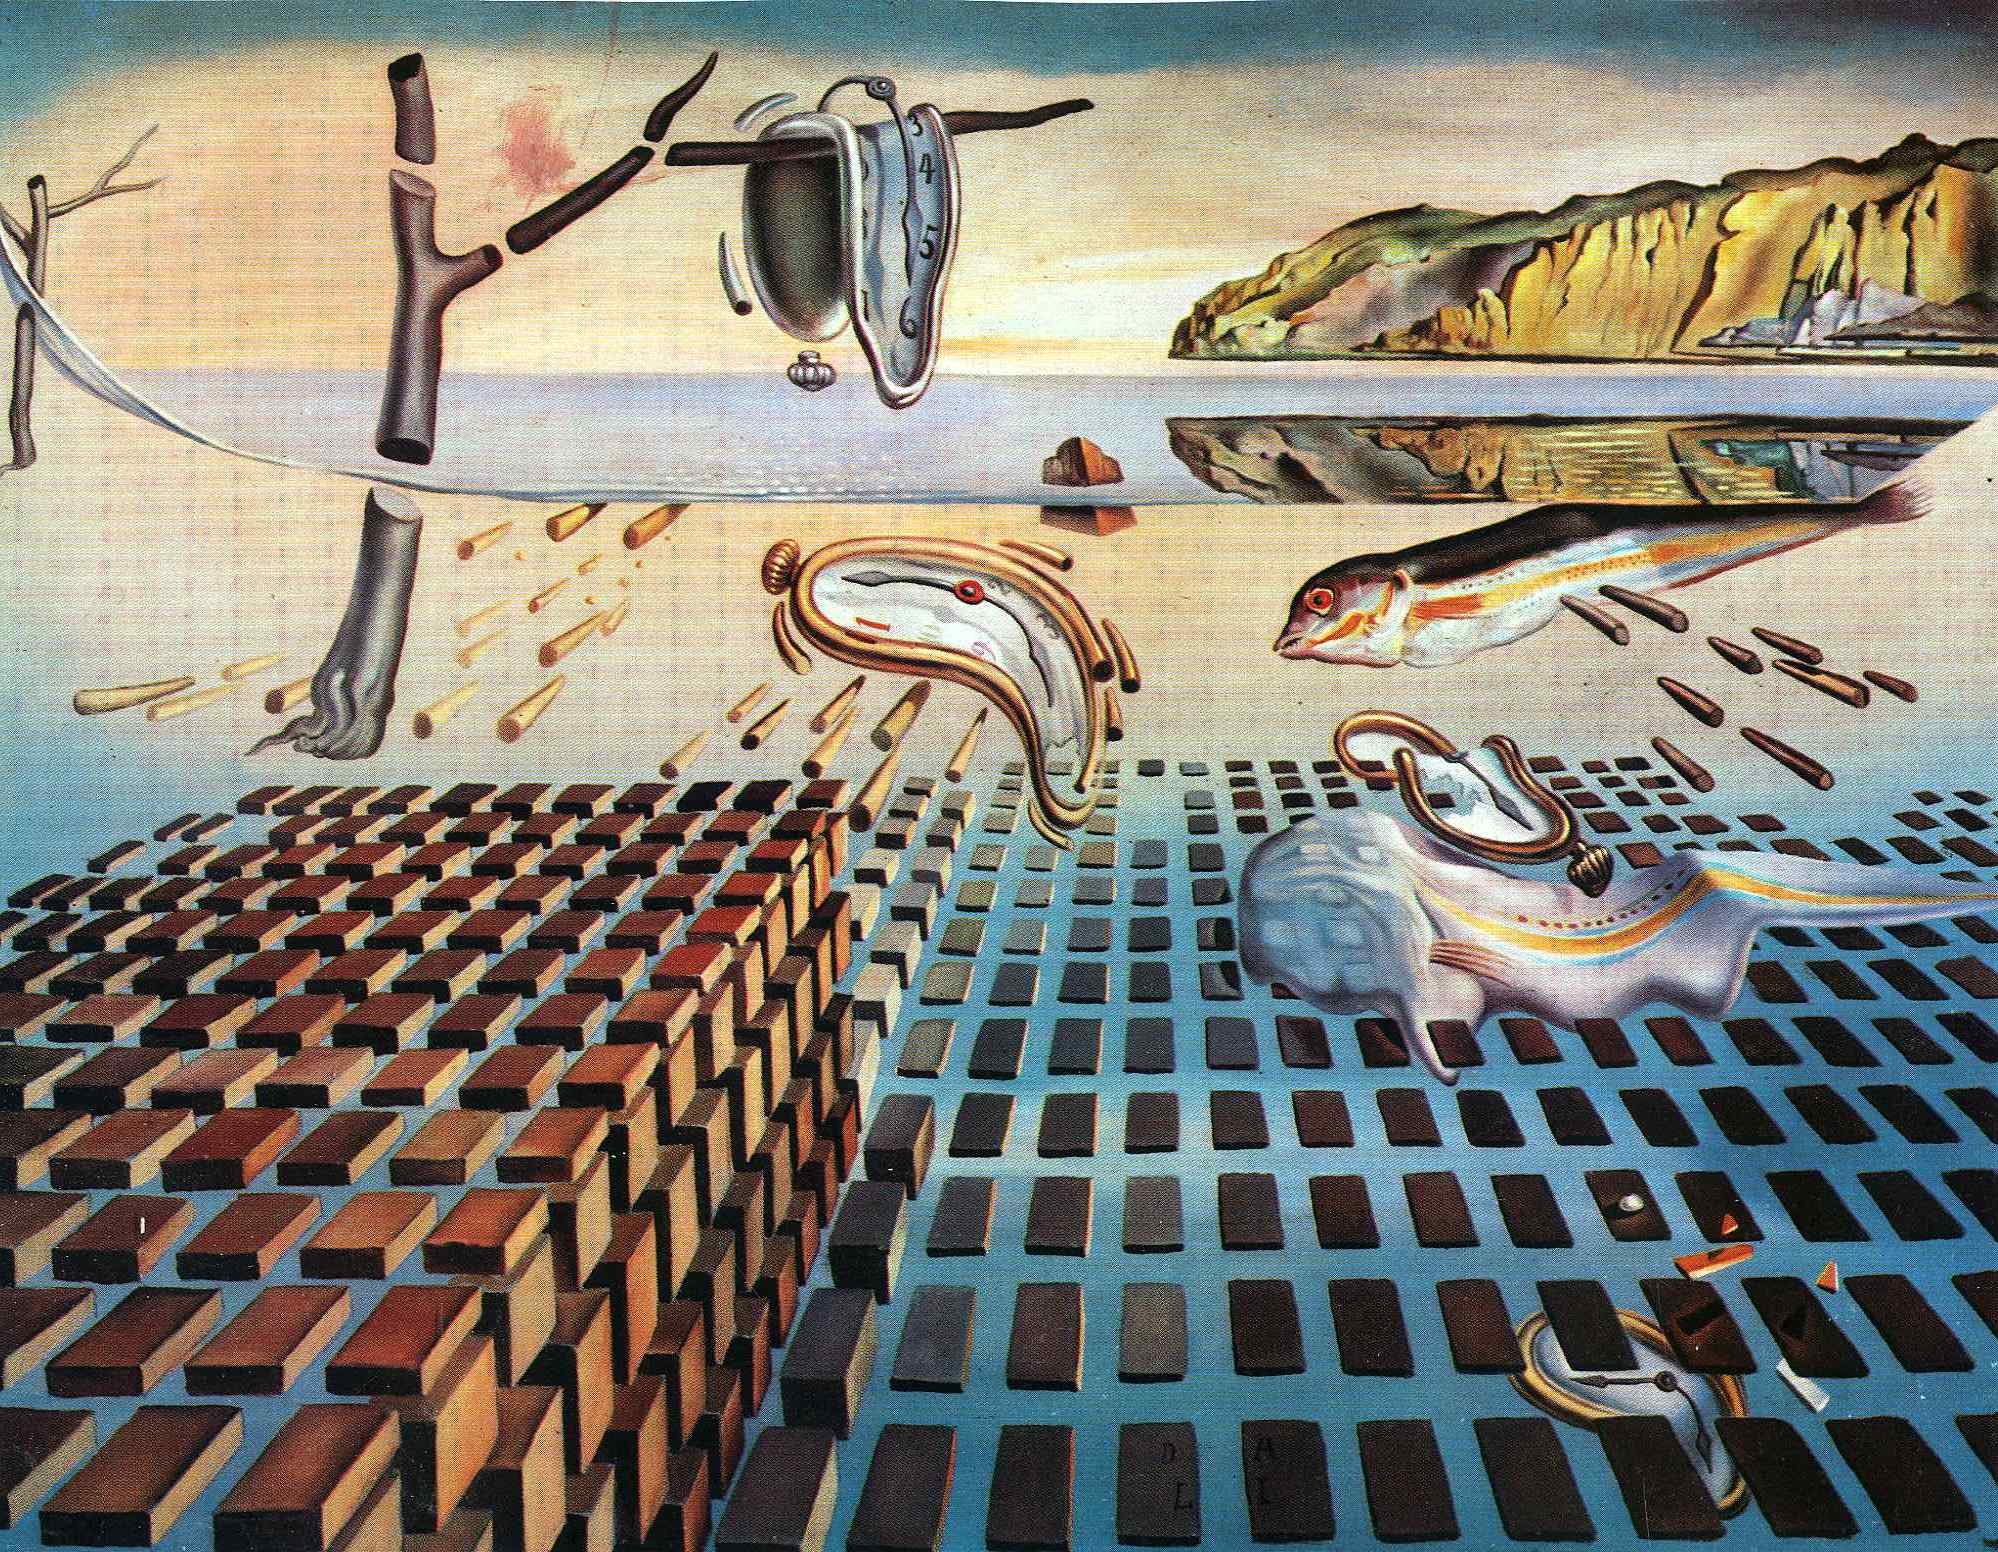
\includegraphics[width=\linewidth]{Figures/painting.jpg}
    \caption{“The Disintegration of the Persistence of Memory” by Salvador Dalí (1952-54).}
    {Image from \href{https://www.wikiart.org/en/salvador-dali/the-disintegration-of-the-persistence-of-memory}{WikiArt}. \copyright\hspace{0.01em} Salvador Dalí.}
    \label{fig.painting}
\end{figure}
\clearpage

\tableofcontents %% Mandatory
%\listoftables                   %% Mandatory if thesis has tables
\listoffigures                  %% Mandatory if thesis has figures
%\listof{Program}{List of Programs} %% Optional
%% Any other lists should come here, i.e.
%% Abbreviation schemes, definitions, lists of formulae, list of
%% schemes, glossary, list of symbols etc.

%\chapter{Dedication} %% Optional
%The dedication is usually quite short, and is a personal rather than
%an academic recognition.  The \emph{Dedication} does not have to be
%titled, but it must appear in the table of contents.  If you want to
%skip the chapter title but still enter it into the Table of Contents,
%use this command \verb|\chapter[Dedication]{}|.

%Note that this section is the last of the preliminary pages (with
%lowercase Roman numeral page numbers).  It must be placed
%\emph{before} the \verb|\mainmatter| command.  After that, Arabic
%numbered pages will begin.

% Any other unusual prefactory material should come here before the
% main body.

% Now regular page numbering begins.
\mainmatter

% Parts are the largest structural units, but are optional.
%\part{Thesis}

% Chapters are the next main unit.
%\chapter{Contents}

\chapter{Introduction}\label{ch.intro}

In quantum mechanics, physical laws are written down as expressions describing total energy called ``Hamiltonians.'' I will use a set of techniques called perturbation theory to study Hamiltonians of the form \(\op{H} = \op{H}_0 + \lambda \op{V}\) where \(\op{H}_0\) is a Hamiltonian that is well understood and \(\lambda\) is very small. I will ask: how much does the entropy change due to \(\lambda \op{V}\)?

I start in this chapter by explaining what entropy is. In Chapter \ref{ch.theory}, I develop the perturbation theory tools that I will need later on. In Chapter \ref{ch.derivation}, I apply these tools to derive general formulae for the change in entropy due to the perturbation \(\lambda \op{V}\). In Chapter \ref{ch.ex}, I discuss a few examples of entropy evolution. Finally, in Chapter \ref{ch.conclusion}, I summarize the results and speculate about future research directions.

The physicist reading this thesis may want to jump straight to Chapter \ref{ch.derivation} because that is where the important results are to be found. The philosopher or casual reader may be more interested in Chapters \ref{ch.intro} and \ref{ch.conclusion}.

\section{What is entropy?}\label{sec.whatisentropy}
\input{"What is Entropy/WIE_whatisentropy"}
\chapter{Theoretical Tools}\label{ch.theory}
\section{Time-dependent perturbation theory in the interaction picture}
\input{"Theoretical Background/BKG_tdpt_density_operator"}
\section{Corrections to eigenvalues of an operator}
\input{"Theoretical Background/BKG_tipt_eigvals"}
\chapter{Growth of Von Neumann Entropy due to a Perturbation}\label{ch.derivation}
\input{"Derivation/DERIVATION"}
\chapter{Examples}\label{ch.ex}
\section{Two qubits}
\input{"Examples/EX_toy"}
\section{Scattering}
\input{"Examples/EX_scattering"}
\chapter{Conclusion}\label{ch.conclusion}
\emph{To be added...}


%% This file is setup to use a bibtex file sample.bib and uses the
%% plain style.  Other styles may be used depending on the conventions
%% of your field of study.
%%
%%% Note: the bibliography must come before the appendices.
%\bibliographystyle{JHEP}
\bibliographystyle{plainnat}
% \bibliographystyle{unsrt}
%\bibliographystyle{acm}
\bibliography{references}
%\printbibliography  %[heading=none, keyword=OWN]
%% Use this to reset the appendix counter.  Note that the FoGS
%% requires that the word ``Appendices'' appear in the table of
%% contents either before each appendix lable or as a division
%% denoting the start of the appendices.  We take the latter option
%% here.  This is ensured by making the \texttt{appendicestoc} option
%% a default option to the UBC thesis class.

%%% If you only have one appendix, please uncomment the following line.
% \renewcommand{\appendicesname}{Appendix}
%\appendix
%\chapter{First Appendix}
%\input{Appendix1}

%\chapter{Second Appendix}
%Here is the second appendix.

%% This changes the headings and chapter titles (no numbers for
%% example).
\backmatter

%% Indices come here if you have them.








    %\url{http://www.grad.ubc.ca/current-students/dissertation-thesis-preparation}\\
   

\end{document}
\endinput
%%
%% End of file `ubcsample.tex'.
